%!TEX TS-program = xelatex

% Шаблон документа LaTeX создан в 2018 году
% Алексеем Подчезерцевым
% В качестве исходных использованы шаблоны
% 	Данилом Фёдоровых (danil@fedorovykh.ru) 
%		https://www.writelatex.com/coursera/latex/5.2.2
%	LaTeX-шаблон для русской кандидатской диссертации и её автореферата.
%		https://github.com/AndreyAkinshin/Russian-Phd-LaTeX-Dissertation-Template

\documentclass[a4paper,14pt]{article}


%%% Работа с русским языком
\usepackage[english,russian]{babel}   %% загружает пакет многоязыковой вёрстки
\usepackage{fontspec}      %% подготавливает загрузку шрифтов Open Type, True Type и др.
\defaultfontfeatures{Ligatures={TeX},Renderer=Basic}  %% свойства шрифтов по умолчанию
\setmainfont[Ligatures={TeX,Historic}]{Times New Roman} %% задаёт основной шрифт документа
\setsansfont{Comic Sans MS}                    %% задаёт шрифт без засечек
\setmonofont{Courier New}
\usepackage{indentfirst}
\frenchspacing

\renewcommand{\epsilon}{\ensuremath{\varepsilon}}
\renewcommand{\phi}{\ensuremath{\varphi}}
\renewcommand{\kappa}{\ensuremath{\varkappa}}
\renewcommand{\le}{\ensuremath{\leqslant}}
\renewcommand{\leq}{\ensuremath{\leqslant}}
\renewcommand{\ge}{\ensuremath{\geqslant}}
\renewcommand{\geq}{\ensuremath{\geqslant}}
\renewcommand{\emptyset}{\varnothing}

%%% Дополнительная работа с математикой
\usepackage{amsmath,amsfonts,amssymb,amsthm,mathtools} % AMS
\usepackage{icomma} % "Умная" запятая: $0,2$ --- число, $0, 2$ --- перечисление

%% Номера формул
%\mathtoolsset{showonlyrefs=true} % Показывать номера только у тех формул, на которые есть \eqref{} в тексте.
%\usepackage{leqno} % Нумерация формул слева	

%% Перенос знаков в формулах (по Львовскому)
\newcommand*{\hm}[1]{#1\nobreak\discretionary{}
	{\hbox{$\mathsurround=0pt #1$}}{}}

%%% Работа с картинками
\usepackage{graphicx}  % Для вставки рисунков
\graphicspath{{images/}}  % папки с картинками
\setlength\fboxsep{3pt} % Отступ рамки \fbox{} от рисунка
\setlength\fboxrule{1pt} % Толщина линий рамки \fbox{}
\usepackage{wrapfig} % Обтекание рисунков текстом

%%% Работа с таблицами
\usepackage{array,tabularx,tabulary,booktabs} % Дополнительная работа с таблицами
\usepackage{longtable}  % Длинные таблицы
\usepackage{multirow} % Слияние строк в таблице
\usepackage{float}% http://ctan.org/pkg/float

%%% Программирование
\usepackage{etoolbox} % логические операторы


%%% Страница
\usepackage{extsizes} % Возможность сделать 14-й шрифт
\usepackage{geometry} % Простой способ задавать поля
\geometry{top=20mm}
\geometry{bottom=20mm}
\geometry{left=20mm}
\geometry{right=10mm}
%
%\usepackage{fancyhdr} % Колонтитулы
% 	\pagestyle{fancy}
%\renewcommand{\headrulewidth}{0pt}  % Толщина линейки, отчеркивающей верхний колонтитул
% 	\lfoot{Нижний левый}
% 	\rfoot{Нижний правый}
% 	\rhead{Верхний правый}
% 	\chead{Верхний в центре}
% 	\lhead{Верхний левый}
%	\cfoot{Нижний в центре} % По умолчанию здесь номер страницы

\usepackage{setspace} % Интерлиньяж
\onehalfspacing % Интерлиньяж 1.5
%\doublespacing % Интерлиньяж 2
%\singlespacing % Интерлиньяж 1

\usepackage{lastpage} % Узнать, сколько всего страниц в документе.

\usepackage{soul} % Модификаторы начертания

\usepackage{hyperref}
\usepackage[usenames,dvipsnames,svgnames,table,rgb]{xcolor}
\hypersetup{				% Гиперссылки
	unicode=true,           % русские буквы в раздела PDF
	pdftitle={ПРОЕКТИРОВАНИЕ И РАЗРАБОТКА ЭЛЕКТРОННОЙ СИСТЕМЫ ДЛЯ ДОПОЛНИТЕЛЬНОГО ОБРАЗОВАНИЯ СО ШКОЛЬНИКАМИ},   % Заголовок
	pdfauthor={Подчезерцев Алексей, Солодянкин Андрей},      % Автор
	pdfsubject={ПРОЕКТИРОВАНИЕ И РАЗРАБОТКА ЭЛЕКТРОННОЙ СИСТЕМЫ ДЛЯ ДОПОЛНИТЕЛЬНОГО ОБРАЗОВАНИЯ СО ШКОЛЬНИКАМИ},      % Тема
	pdfcreator={Подчезерцев Алексей, Солодянкин Андрей}, % Создатель
	pdfproducer={Подчезерцев Алексей, Солодянкин Андрей}, % Производитель
	pdfkeywords={МКР} {Moodle} {МИЭМ} {ВШЭ}, % Ключевые слова
	colorlinks=true,       	% false: ссылки в рамках; true: цветные ссылки
	linkcolor=black,          % внутренние ссылки
	citecolor=black,        % на библиографию
	filecolor=magenta,      % на файлы
	urlcolor=black           % на URL
}
\makeatletter 
\def\@biblabel#1{#1. } 
\makeatother
\usepackage{cite} % Работа с библиографией
%\usepackage[superscript]{cite} % Ссылки в верхних индексах
%\usepackage[nocompress]{cite} % 
\usepackage{csquotes} % Еще инструменты для ссылок

\usepackage{multicol} % Несколько колонок

\usepackage{tikz} % Работа с графикой
\usepackage{pgfplots}
\usepackage{pgfplotstable}

% ГОСТ заголовки
\usepackage[font=small]{caption}
%\captionsetup[table]{justification=centering, labelsep = newline} % Таблицы по правобу краю
%\captionsetup[figure]{justification=centering} % Картинки по центру


\newcommand{\tablecaption}[1]{\addtocounter{table}{1}\small \begin{flushright}\tablename \ \thetable\end{flushright}%	
\begin{center}#1\end{center}}

\newcommand{\imref}[1]{рис.~\ref{#1}}

\usepackage{multirow}
\usepackage{spreadtab}
\newcolumntype{K}[1]{@{}>{\centering\arraybackslash}p{#1cm}@{}}


\usepackage{xparse}
\ExplSyntaxOn
\DeclareExpandableDocumentCommand{\juliandate}{ m m m }
{
	\juliandate_calc:nnnn { #1 } { #2 } { #3 } { \use:n }
}
\NewDocumentCommand{\storejuliandate}{ s m m m m }
{
	\IfBooleanTF{#1}
	{
		\juliandate_calc:nnnn { #3 } { #4 } { #5 } { \cs_set:Npx #2 }
	}
	{
		\juliandate_calc:nnnn { #3 } { #4 } { #5 } { \cs_new:Npx #2 }
	}
}
\cs_new:Npn \juliandate_calc:nnnn #1 #2 #3 #4 % #1 = day, #2 = month, #3 = year, #4 = what to do
{
	#4 
	{
		\int_eval:n
		{
			#1 +
			\int_div_truncate:nn { 153 * (#2 + 12 * \int_div_truncate:nn { 14 - #2 } { 12 } - 3) + 2 } { 5 } +
			365 * (#3 + 4800 - \int_div_truncate:nn { 14 - #2 } { 12 } ) +
			\int_div_truncate:nn { #3 + 4800 - \int_div_truncate:nn { 14 - #2 } { 12 } } { 4 } -
			\int_div_truncate:nn { #3 + 4800 - \int_div_truncate:nn { 14 - #2 } { 12 } } { 100 } + 
			\int_div_truncate:nn { #3 + 4800 - \int_div_truncate:nn { 14 - #2 } { 12 } } { 400 } -
			32045
		}
	}
}

\tl_new:N \l__juliandate_g_tl
\tl_new:N \l__juliandate_dg_tl
\tl_new:N \l__juliandate_c_tl
\tl_new:N \l__juliandate_dc_tl
\tl_new:N \l__juliandate_b_tl
\tl_new:N \l__juliandate_db_tl
\tl_new:N \l__juliandate_a_tl
\tl_new:N \l__juliandate_da_tl
\tl_new:N \l__juliandate_y_tl
\tl_new:N \l__juliandate_m_tl
\tl_new:N \l__juliandate_d_tl
\int_new:N \l_juliandate_day_int
\int_new:N \l_juliandate_month_int
\int_new:N \l_juliandate_year_int

\cs_new:Npn \__juliandate_set:nn #1 #2
{
	\tl_set:cx { l__juliandate_#1_tl } { \int_eval:n { #2 } }
}
\cs_new:Npn \__juliandate_use:n #1
{
	\tl_use:c { l__juliandate_#1_tl }
}
\cs_new_protected:Npn \juliandate_reverse:n #1
{
	\__juliandate_set:nn { g }
	{ \int_div_truncate:nn { #1 + 32044 } { 146097 } }
	\__juliandate_set:nn { dg }
	{ \int_mod:nn { #1 + 32044 } { 146097 } }
	\__juliandate_set:nn { c }
	{ \int_div_truncate:nn { ( \int_div_truncate:nn { \__juliandate_use:n { dg } } { 36524 } + 1) * 3 } { 4 } }
	\__juliandate_set:nn { dc }
	{ \__juliandate_use:n { dg } - \__juliandate_use:n { c } * 36524 }
	\__juliandate_set:nn { b }
	{ \int_div_truncate:nn { \__juliandate_use:n { dc } } { 1461 } }
	\__juliandate_set:nn { db }
	{ \int_mod:nn { \__juliandate_use:n { dc } } { 1461 } }
	\__juliandate_set:nn { a }
	{ \int_div_truncate:nn { ( \int_div_truncate:nn { \__juliandate_use:n { db } } { 365 } + 1) * 3 } { 4 } }
	\__juliandate_set:nn { da }
	{ \__juliandate_use:n { db } - \__juliandate_use:n { a } * 365 }
	\__juliandate_set:nn { y }
	{
		\__juliandate_use:n { g } * 400 + 
		\__juliandate_use:n { c } * 100 + 
		\__juliandate_use:n { b } * 4 + 
		\__juliandate_use:n { a }
	}
	\__juliandate_set:nn { m }
	{ \int_div_truncate:nn { \__juliandate_use:n { da } * 5 + 308 } { 153 } - 2 }
	\__juliandate_set:nn { d }
	{ \__juliandate_use:n { da } - \int_div_truncate:nn { (\__juliandate_use:n { m } + 4) * 153 } { 5 } + 122 }
	\int_set:Nn \l_juliandate_year_int
	{ \__juliandate_use:n { y } - 4800 + \int_div_truncate:nn { \__juliandate_use:n { m } + 2 } { 12 } }
	\int_set:Nn \l_juliandate_month_int
	{ \int_mod:nn { \__juliandate_use:n { m } + 2 } { 12 } + 1 }
	\int_set:Nn \l_juliandate_day_int
	{ \__juliandate_use:n { d } + 1 }
}
\cs_generate_variant:Nn \juliandate_reverse:n { x }

\NewDocumentCommand{\showday}{ m }
{
	\juliandate_reverse:n { #1 }
	\int_to_arabic:n { \l_juliandate_day_int }-
	\int_to_arabic:n { \l_juliandate_month_int }-
	\int_to_arabic:n { \l_juliandate_year_int }
}

\NewDocumentCommand{\tomorrow}{ }
{
	\group_begin:
	\juliandate_reverse:x { \juliandate_calc:nnnn { \day + 1 } { \month } { \year } { \use:n } }
	\day = \l_juliandate_day_int
	\month = \l_juliandate_month_int
	\year = \l_juliandate_year_int
	\today
	\group_end:
}
\NewDocumentCommand{\tomorrowof}{ m m m }
{
	\group_begin:
	\juliandate_reverse:x { \juliandate_calc:nnnn { #1 + 1 } { #2 } { #3 } { \use:n } }
	\day = \l_juliandate_day_int
	\month = \l_juliandate_month_int
	\year = \l_juliandate_year_int
	\today
	\group_end:
}
\ExplSyntaxOff
\begin{document} % конец преамбулы, начало документа
\begin{titlepage}
	\begin{center}
		ФЕДЕРАЛЬНОЕ  ГОСУДАРСТВЕННОЕ АВТОНОМНОЕ \\
		ОБРАЗОВАТЕЛЬНОЕ УЧРЕЖДЕНИЕ ВЫСШЕГО ОБРАЗОВАНИЯ\\
		«НАЦИОНАЛЬНЫЙ ИССЛЕДОВАТЕЛЬСКИЙ УНИВЕРСИТЕТ\\
		«ВЫСШАЯ ШКОЛА ЭКОНОМИКИ»
	\end{center}
	
	\begin{center}
		\textbf{Московский институт электроники и математики}
		
		\textbf{Им. А.Н.Тихонова НИУ ВШЭ}
	\end{center}
	\vspace{1ex}	
	\begin{center}
		Солодянкин Андрей Александрович, группа БИВ172\\
		Подчезерцев Алексей Евгеньевич, группа БИВ172
	\end{center}	
	\vspace{1ex}
	\begin{center}
		\textbf{ТЕХНИЧЕСКОЕ ЗАДАНИЕ\\
		ПО МЕЖДИСЦИПЛИНАРНОЙ КУРСОВОЙ РАБОТЕ
	}
	\end{center}	
	\vspace{2ex}
	\begin{center}
		по теме «Проектирование и разработка электронной системы для дополнительного образования со школьниками»\\
	\end{center}
	\vspace{2ex}
	\begin{center}
%	Дата сдачи отчета: \today
	\end{center}
	\vspace{2ex}
	\vfill
	\begin{center}
		Москва \the\year г.
	\end{center}
\end{titlepage}

\section*{Аннотация}

%Количество страниц работы: \getlastpage, иллюстраций: \totalfigures, таблиц: \totaltables, источников: \LastBib.

\pagebreak

\section*{Annotation}

%Total number of pages is \getlastpage, figures: \totalfigures, tables: \totaltables, cite sources: \LastBib.
\pagebreak

\tableofcontents
\pagebreak

\section*{Введение}

% Начало введения

% Актуальность

% Новизна

% Объект

% Предмет

% Цель

% Задачи

% Значимость

% Личный вклад

% Конец введения

\pagebreak

% ==============================================================================
% Начало Г1

\section{Обзор и анализ предметной области}

% Comment - надо аккуратно перенести часть текста во 2 главу, чтобы GIT не ругался

\subsection{Состояние предметной области}

Важной частью современного образования является дополнительные образовательные программы, которые направлены на разностороннее развитие личных качеств.
Секции, кружки по интересам, образовательные курсы получили широкое распространение во многих странах мира.
Некоторые учебные программы финансируются государством, другие привлекают школьников или студентов для дальнейшей учёбы или работы.

Современный курс может носить как дистанционный, так и очный характер, однако в любом случае необходимо организовать данный процесс.
Преподавателям и руководителям требуется контролировать запись и посещаемость, распространение справочного материала, проводить срез знаний, проверять работы, вести учёт оценок и выполнять множество других однотипных действий.
Логичным решением данной проблемы есть автоматизация данного процесса с использованием программных средств.

Данный подход широко используется в современном образовании. В частности, многие организации используют собственные системы контроля образовательного процесса или подключаются к уже готовым решениям.

% Г1 - детальное и подробное описание существующих технологий

% Г1 - детальное и подробное описание аналогичных технологических решений

% Г1 - анализ технологий

% Г1 - Выбор Решения - таблица сравнения

% Г1 - Выводы и заключение

% Конец Г1
% ==============================================================================
% Начало Г2

% Методы решения

\section{Обзор и анализ методов решения}

\subsection{Анализ существующих решений}

%Существует огромное количество систем управления обучением, 

%В последнее время появилось огромное количество систем для управления образованием. 
Для сравнения были выбраны следующие варианты:

\begin{itemize}
	\item iSpring Online LMS
	\item Moodle	
	\item edx
	\item LMS HSE
	
\end{itemize}

% Детальное описание

\subsubsection{iSpring Online LMS}

Аналогов iSpring Online LMS существует очень много.
%Их объединяет следующие преимущества этих систем: простота в установке и управлении
К основными чертам таких систем можно отнести:
\begin{itemize}
	\item простота в установке
	\item простота в управлении	
	\item профессиональная техническая поддержка.
\end{itemize}

При этом у них присутствуют следующие недостатки:
\begin{itemize}
	\item отсутствие кастомизации
	\item стоимость системы
\end{itemize} 

\subsubsection{LMS eFront }

\begin{itemize}
	\item Чёткая вёрстка веб-страниц, стабильная работа программной оболочки 
	\item Подробные отчёты о деятельности пользователей с гибкой фильтрацией	
	
\end{itemize} 

Недостатки системы:

\begin{itemize}
	\item Относительно небольшое количество инструментов для создания учебных материалов
	\item Относительно мало дополнительных модулей
	\item Малое сообщество пользователей
	
	
\end{itemize} 

\subsubsection{Moodle}

Moodle - крупнейшая и самая популярная система управления курсами, которая активно развивается с 2002 года. Важными преимуществами этой системы являются:

\begin{itemize}
	\item бесплатность системы
	\item Неограненный возможности кастомизации
	\item Наличие широкого функционала для обеспечения процесса обучения (есть почти всё)
	\item Бесплатная, с открытым исходным кодом
	\item Большое онлайн-сообщество на официальном сайте
	
\end{itemize} 

Минусы системы:

\begin{itemize}
	\item Сложна для освоения	
\end{itemize} 


\subsubsection{Open edX} 

Платформа Open edX была создана Массачусетским технологическим институтом совместно с Гарвардским университетом.
Данная платформа позволяет создавать массовые онлайн курсы, ориентированные для широкой аудитории.

К достоинствам данного решения можно отнести:

\begin{itemize}
	\item Открытый исходный код платформы
	\item Разнообразие плагинов для расширения функционала
	\item Большое сообщество разработчиков
\end{itemize}

Недостатки:

\begin{itemize}
	\item Система ориентирована на дистанционное обучение
	\item Сложность с интеграцией с существующими проектами образовательного учреждения
\end{itemize}

\subsubsection{Собственное решение} 

\textbf{Написать решение с <<Нуля>>} часто рассматривается при проектировании.
Оно позволит создать продукт с функционалом, наиболее подходящим к желанию заказчика.

Достоинства подхода:

\begin{itemize}
	\item Возможность создать продукт с максимальным соответствием требованиям
	\item Отсутствие зависимостей от сторонних готовых CMS 
\end{itemize}

Однако, данный подход содержит существенный недостаток: высокая стоимость разработки (в человеко-часах).
Разработчикам придётся создать весь функционал, который существует в готовых решениях,  и ещё добавить связанный с конкретной задачей.
Кроме того, не будет достаточно времени и ресурсов для полного тестирования системы.

% Анализ методов

% TODO совпадение с предыдущим пунктом?

% Выбор метода

\begin{landscape}
	\begin{table}[!h]
		\begin{center}
			\begin{flushleft}
				\tablecaption{Сравнение основных систем}
			\end{flushleft}
			
			\begin{tabular}{|l|l|l|l|l|l|}
				\hline
				& iSpring Online LMS & LMS eFront & Moodle & Open edX & Собственное решение \\ \hline
				Бесплатно                              & -                  & +          & +      & +        & +                   \\ \hline
				Малое время разработки                 & +                  & +          & +      & +        & -                   \\ \hline
				Наличие широкого сообщества            & техподдержка       & ±          & +      & +        & -                   \\ \hline
				Возможность кастомизации               & -                  & ±          & ±      & ±        & +                   \\ \hline
				Простота разработки                    & -                  & ±          & +      & +        & -                   \\ \hline
				Простота обслуживания                  & +                  & ±          & ±      & ±        & +                   \\ \hline
				Надежность                             & +                  & +          & +      & +        & -                   \\ \hline
				Ориентация на традиционное образование & +                  & +          & +      & -        & +                   \\ \hline
			\end{tabular}
		\end{center}
	\end{table}
\end{landscape}

% Заключение и выводы

% Конец Г2
% ==============================================================================
% Начало Г3

% Модели

% Методы

% Алгоритмы

% Схемы

% UML

% Выводы

% Конец Г3
% ==============================================================================
% Начало Г4

\section{Практическая реализация}
% Описание решения
\subsection{Подготовка окружения}

Для разработки была взята последняя стабильная версия 3.6.1 на GitHub, однако история разработки была сброшена, так как проект Moodle имеет слишком большую историю разработки и более 90 тысяч коммитов только в главной ветке.
Для хостинга кода был создан приватный репозиторий на GitHub.

В качестве сервера был использован уже имеющийся хостинг VPS DigitalOcean с сервером в Лондоне на минимальном тарифном плане (1 vCPU, 1 ГБ RAM, 25 ГБ SSD), на котором были уже установлены СУБД MySQL и web сервер NGINX для других проектов.
Было выделено доменное имя 3 уровня \url{lms.asciishell.site} на собственном домене.
Был создан новый unix пользователь для работы с новым сервисом, настроен доступ к репозиторию по ключу.
Кроме того, для успешной работы Moodle понадобилось установить php интерпретатор и apache. 
После потребовалось настроить NGINX прокси и apache для совместной работы, сконфигурировать LetsEncrypt для выдачи и автоматического обновления сертификата безопасности сайта.
Для разработки был использован Open Server с MySQL и php.
На данном этапе первичная настройка была окончена, чего было достаточно для разработки и тестирования на реальном сервере.

\subsection{Установка плагинов}

Многий функционал в Moodle добавляется и настраивается с помощью специальных пакетов -- плагинов -- которые расширяют функционал приложения.
Moodle имеет богатую библиотеку плагинов, позволяющие решить практически любую типовую задачу.

В первую очередь был установлен и настроен \textbf{CodeRunner} и зависимые плагины.
Данный плагин позволяет создавать вопросы с проверкой программного кода ученика на многих языках, в том числе на Python, C++ и JavaScript.

Для большего удобства дальнейшей работы были установлены расширения для подсветки исходного кода для повышения удобочитаемости и привитию привычки к качественному коду у учеников.

Кроме того, были добавлены плагины с вопросами на упорядочивание данных и соотношения для увеличения возможностей преподавательского состава проверять знания учащихся.

\subsection{Настройка почты}

Одна из функций нашей платформы -- рассылка почты.
Данный функционал присутствует практически в каждом современном сайте с регистрацией пользователя.
С помощью почты пользователь может получать уведомления от учителя, администратора, взаимодействовать с другими пользователями.

В качестве сервера почты был выбран Яндекс.Коннект, который предоставляет удобный и понятный интерфейс для управления записями доменного имени, а так же не менее простой и бесплатный сервис по настройке почты для своего домена (Рис. \ref{img:yandex}).
Был создан почтовый ящик, с которого необходимо производить рассылку корреспонденции (Рис. \ref{img:miemMail}), далее установлен и настроен почтовый сервер postfix для приёма писем с Moodle и пересылкой их на сервера Яндекса.
В Moodle сервером получателем был указан localhost.

\begin{figure}[H]
	\centering
	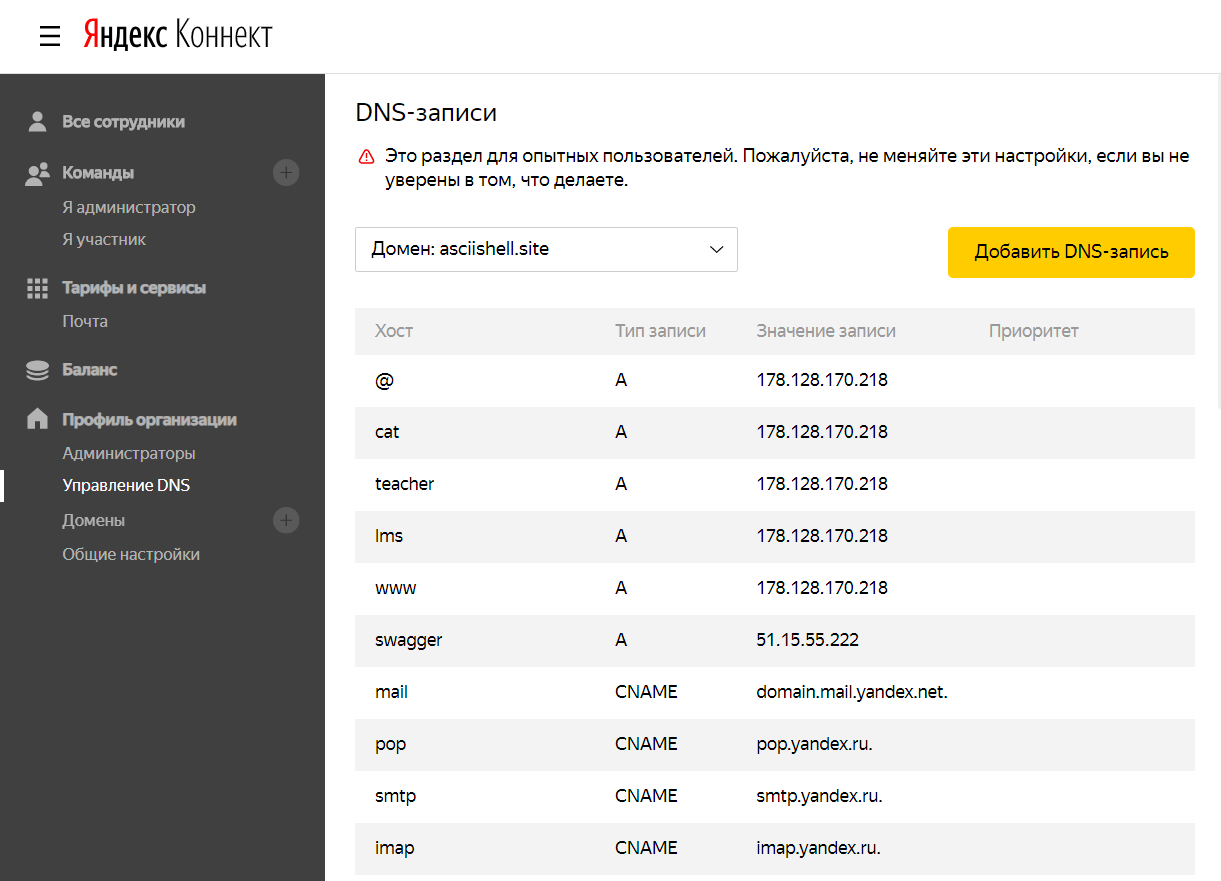
\includegraphics[width=0.7\linewidth]{image/yandex_connect}
	\caption{Интерфейс администратора домена Яндекс.Коннект}
	\label{img:yandex}
\end{figure}

\begin{figure}[H]
	\centering
	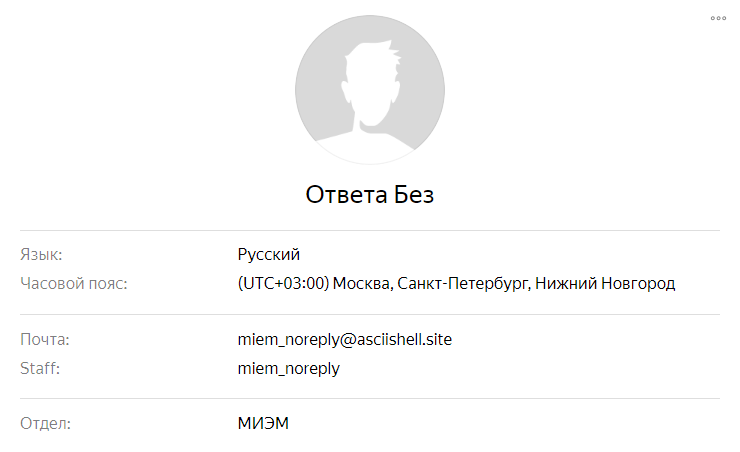
\includegraphics[width=0.7\linewidth]{image/yandex_miem}
	\caption{Учётная запись почтовой рассылки}
	\label{img:miemMail}
\end{figure}

% Описание экспериментов

% Демонстрация

% Анализ результатов

% Подтверждение актуальности

% Выводы и заключение

% Конец Г4
% ==============================================================================
% Начало заключения

% Результаты

% Научная новизна и практическая значимость

% Личный вклад каждого соавтора работы, даже если автор 1

% Ваши выводы

% Предполагаемое применение полученных результатов

% Направление дальнейших исследований (перспективы дальнейшего развития работы)

% Конец заключения
% ==============================================================================
\end{document} % конец документа

